\section{Introducción}
El signo de Hoffmann es un reflejo muscular que se produce al percutir suavemente el lecho ungueal del dedo medio o índice como se muestra en la figura \ref{fig:Hoffman_sign}, produciéndose un movimiento de flexión involuntario del pulgar cuando el examinador hace girar la uña del dedo medio hacia abajo. Fue propuesto por primera vez por Johann Hoffmann, un neurólogo alemán, a finales del siglo XIX. Y descrito por primera vez gracias a Hans Curschmann, uno de sus asistentes, en 1911\cite{ BENDHEIM}. Su presencia puede indicar una lesión en los tractos corticoespinales, vías neuronales que conectan la corteza cerebral con la médula espinal. 


\begin{figure}[h!]
	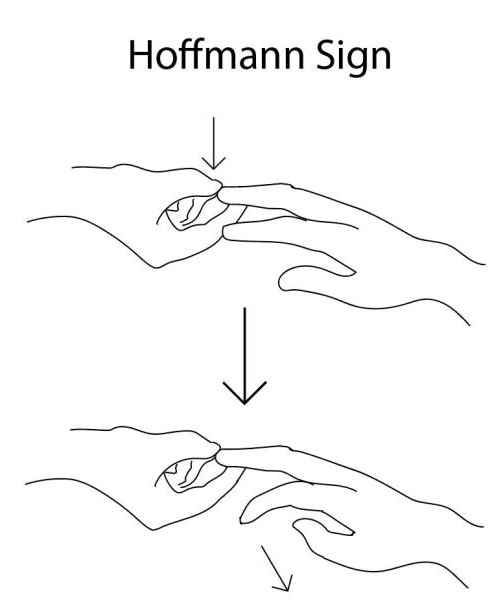
\includegraphics[width=0.35\textwidth]{figures/Kabir_Hoffmann__Sign.jpg}
	\caption{Signo de Hoffmann. Este diagrama muestra un signo de Hoffmann positivo, una parte estándar del examen neurológico común. Contribución de R Kabir, MD}
	\label{fig:Hoffman_sign}
\end{figure}


No obstante es importante destacar que el signo de Hoffman es un fenotipo y no una enfermedad en sí, se ha descubierto que hasta el 3\% de la población presenta un signo de Hoffmann positivo sin que haya compresión de la médula. Este reflejo está asociado a 12 enfermedades diferentes\cite{whitney}.